
\clearpage
\section{Testing the UDAPL library}
Here we describe what we did with the uDAPL on the IB cluster.

\subsection{Overview}

uDAPL is a user-level direct access API
developed by DAT collaborative {\tt http://www.datcollaborative.org}.

The main objectivity of uDAPL is to provide a transport and platform independent 
API for data communication between nodes.
The main features of uDAPL are:
\begin{compactitem}[$\bullet$]
 \item {\bf point-to-point} connection, advanced connection management; 
 \item management of {\bf memory} buffers;
 \item {\bf zero-copy} data transfer;
 \item {\bf message} and {\bf RDMA} data transfer. 
\end{compactitem} 


\subsection{Installation on IB test cluster}

The mellanox IB Gold distribution v 1.8.0 for Linux was installed on the Infiniband-cluster\\
(see {\tt https://docs.mellanox.com/dm/ibgold/ReadMe.html} for more details).
Source package and documentation can be found in {\tt /usr/oub/ibgd}.

The package is installed localy for each node in {\tt /usr/local/ibgd}. 
The complete set of components was installed. 
To compile Mellanox IB Gold, package {\tt termcap-2.0.8-879.i586.rpm} (from SuSE distribution) 
was installed on each machine.

After installation several configuration files where modified:

\begin{table}[htb]
\begin{center}

\caption{List of modified configuration files}

\begin{tabular}{|l|l|}\hline

 {\tt /etc/infiniband/ifcfg-ib0}   & here correct IP address for Infiniband should be set \\ \hline
 {\tt /etc/infiniband/openib.conf} & set modules, which should be loaded, enable uDAPL (default - no) \\ \hline
 {\tt /etc/opensm.conf}            & on master node ONBOOT=yes should be set \\ \hline

\end{tabular}
\end{center}
\end{table}

IP over IB (IPoIB) was configured in following way:

\begin{table}[htb]
\begin{center}

\caption{List of IP adresses in InfiniBand network}

\begin{tabular}{|l|l|}\hline
 Host     & IP adress  \\ \hline
 master   & 11.0.0.1   \\ \hline
 node01   & 11.0.0.2   \\ \hline
 node02   & 11.0.0.3   \\ \hline
 node03   & 11.0.0.4   \\ \hline
\end{tabular}
\end{center}
\end{table}


\subsection{Running of standard InfiniBand transport tests}

Included in the Mellanox IB Gold distribution are test suites for MPI and uDAPL stack.
With them one can test bandwidth and latency for both protocols.

\subsubsection{MPI tests}
They are located in {\tt /usr/local/ibgd/mpi/osu/gcc/tests} (which can be accessed as {\tt \$MPITESTS}).

1. MPI bandwidth test (repeat=1000, packetsize=1000000):\\
{\tt mpirun\_rsh -np 2 node01 node02 `echo \$MPITESTS`/osu-tests/bw 1000 1000000}\\
Result is:
\begin{verbatim}
1000000 952.753887 Mb/s
\end{verbatim}

2. MPI latency test:\\
{\tt mpirun\_rsh -np 2 node01 node02 `echo \$MPITESTS`/osu-tests/lt 1000 16}\\
Result is ($\mu$s):
\begin{verbatim}
16      4.025500
\end{verbatim}

3. Presta bandwidth tests between two nodes:\\
{\tt mpirun\_rsh -np 2 node01 node02 `echo \$MPITESTS`/presta1.2/com -o 100}\\
Result is:
\begin{verbatim}
Max Unidirectional Bandwith :  953.18 Mb/s for message size of 8.4 Mbytes
Max  Bidirectional Bandwith : 1479.47 Mb/s for message size of 0.5 Mbytes
\end{verbatim}

4. Presta latency test:\\
{\tt mpirun\_rsh -np 2 node01 node02 `echo \$MPITESTS`/presta1.2/laten -o 1000}\\
Result is ($\mu$s):
\begin{verbatim}
Maximum latency = 4.947 
\end{verbatim}

5. Presta test for MPI\_Allreduce operation:\\
{\tt mpirun\_rsh -np 4 master n1 n2 n3 `echo \$MPITESTS`/presta1.2/allred 10 10 100}\\
Result is (times in $\mu$):
\begin{verbatim}
MPI Allreduce test
  for 4 MPI processes, message size 32 bytes, 
  10 operations per sample, 100 samples

  Wtick resolution           :      10.000
  Time between Allreduce     :       7.000

  Mean Compute Loop Time     :      65.270
  Ticks per Compute Loop     :           7
  Mean Op Loop Time          :     179.200
  Ticks per Op Loop          :          18

  Op mean                    :      11.393
\end{verbatim}

6. Presta MPI Global-Op benchmark:\\
{\tt mpirun\_rsh -np 4 master n1 n2 n3 `echo \$MPITESTS`/presta1.2/globalop}\\
Result is ($\mu$):
\begin{verbatim}
Average elapsed run time was    4.21
\end{verbatim}

7. Pallas tests:\\
{\tt mpirun\_rsh -np 2 node01 node02 `echo \$MPITESTS`/PMB2.2.1/PMB-MPI1}\\
Results:\\
Are not listed here, can be found on daq4fair wiki.

\subsubsection{uDAPL tests}

The test suite was downloaded from DAT collaborative web site. 
Seems to be, the same is included in the Mellanox as well.\\
Currently the example is compiled in {\tt /u/linev} directory, but also can be accessed by other users.\\
To run the example copy executable from \\
{\tt /u/linev/dapl/test/dapltest/udapl/Target/dapltest}\\
 to home directory. On node01 run example as server:

{\tt ./dapltest -T S -D ib0}

On node02 (or any other) run example as client:

{\tt ./dapltest -T T -s 11.0.0.2 -D ib0 -i 1000 -t 2 -w 1 \\
client SR 1048576 server SR 1048576 client RR 100000 client RW 100000}

Crutial here, that correct IP address of server (for node01 it is 11.0.0.2) should be set.

More details about arguments can be found in Readme file.

Results is:
\begin{verbatim}
Server Name: 11.0.0.2
Server Net Address: 11.0.0.2
DT_cs_Client: Starting Test ...
----- Stats ---- : 2 threads, 1 EPs
Total WQE        :    1694.91 WQE/Sec
Total Time       :       4.71 sec
Total Send       :    2097.15 MB -     444.31 MB/Sec
Total Recv       :    2097.15 MB -     444.31 MB/Sec
Total RDMA Read  :     200.00 MB -      42.37 MB/Sec
Total RDMA Write :     200.00 MB -      42.37 MB/Sec
DT_cs_Client: ====== End of Work -- Client Exiting 
\end{verbatim}

\subsection{C++ wrapper for uDAPL fuctionality}
\label{uDAPL-cpp}

uDAPL is a C-based library and has a number of different structures, which should be initialized before 
data transport can be started. To simplify futher development of the uDAPL communication test program, 
 C++ wrapper classes for most important uDAPL functions and structures are implemented. These are:

\begin{compactitem}[$\bullet$]
 \item {\bf TEndPoint} - contains handle and attributes of single point-to-point conection; 
 \item {\bf TMemorySpace} - memory region plus neccessary structures for uDAPL zero-copy data transfer; 
 \item {\bf TMemoryPool} - pool of TMemorySpace objects;
 \item {\bf TBasic} - combines necessary structures and functions for uDAPL communications.
\end{compactitem} 

Central class is TBasic. It provides following functionality:

\begin{compactitem}[$\bullet$]
 \item initialisation / finalisation of different uDAPL structures, required on each node; 
 \item high-level method for establishing connection with other nodes; 
 \item allocation of memory / memory pools; 
 \item sending / receivng data over uDAPL connection; 
 \item handling RDMA read / write operations.
\end{compactitem} 

\subsection{uDAPL test application}
\label{uDAPL-testapp}

Using the C++ wrapper classes for uDAPL a test application was implemented. 
The same executable should run on each node.
One executable became master role, all other run as slaves.
The master drives the complete test, sending commands to each slave one by one. 
Slaves normally should wait for next command and, when it arrives, start execution.
But when real test is executed (for instance, all-to-all data transfer test), 
absolutely the same code will run on master and slaves. 
When a command (running test) is completed, the slave again switched to waiting state 
while master decides which command should be executed next.
The command list is defined in the test application and includes:
\begin{compactitem}[$\bullet$]
 \item time synchronisation; 
 \item sleep; 
 \item exit; 
 \item all-to-all communication test with message data transfers; 
 \item all-to-all communication test with RDMA data transfer.
 \item chaotic (non-scheduled) data transfer.
\end{compactitem} 

The test executable should be started practically simultanious, 
while during initialisation phase connection with all other nodes should be established.
After that slaves just going to command waiting loop, while on master the 
programmed test sequence is executed.
Typically such sequence includes different combinations of packet size, schedule pattern, 
queues size and so on. The main task of such tests was to determine the maximum data transfer rate 
achievable with an InfiniBand network with different setups.

\subsection{Time synchronisation}

Time synchronisation between nodes is required to implement a scheduled data transfer. 
InfiniBand provides 10 Gbit/sec data rate. To synchronise the transfer of two packets of 1 KB size
one needs a precision in packet send time of at least 1 $\mu$s. 
It is assumed that at least one or several packets can be buffered in network switches / host adapters.
Therefore a synchronisation better than one packet size is not required. 
For time measurements in a $\mu$s range one can use the PC clock counter. 
In the test application function {\tt ntp\_gettime()} is used. 

But to be able produce synchronous operations on different nodes, the clocks must be synchronised.
For that a small round-trip packet is used. The master sends a small packet with a 
time stamp inside to one of the slaves.
The slave adds its own time stamp value and sends packet back. 
When the master receives such packet, it can determine how long the round-trip took place 
and what was a middle 
time on master and slave sides. As a result, it can calculate the
time difference between the time on master and slave nodes. 
Typical round-trip times are about $29\pm0.5~\mu$s. 
Such round-trip packets are sent up to 100 times to calculate the 
average time difference and to achieve a precision of about 0.2 $\mu$s.
At the end the master sends a packet to the slave with a time correction value, which should be
used to calculate correct time stamps on the slave side.

Time measurements with {\tt ntp\_gettime()} function use the CPU clock.
On different nodes one can expect a deviation between the CPU clock frequency.
On our test cluster 10 s after synchronisation such deviation leads to ~200 $\mu$s 
difference between nodes and 
this difference poportianally grows with time. 
It means, that the observed difference in CPU clock is $10^{-5}$.
This is a very significant value relative to required precision of 1 $\mu$s 
during at least 100 s or $10^{-8}$. 
To compensate this effect, a time scale factor must be applied. 
Therefore the master repeats time synchronisation after
10 seconds and defines a time scale factor for each slave. 
With the last round-trip packet this factor is sent to slave.

After the time synchronisation procedure the time stamp 
on each node is calculated by the following equation:

\begin{equation}
\label{eq-CalibrTime}
T_{synch} = (T_{clockl} - T_{0}) * Coef + Shift,
\end{equation}

$T_{synch}$ : synchronised time\\
$T_{clockl}$ : local CPU clock\\ 
$Coef$ : time coefficient, applied at $T_{0}$\\
$Shift$ : time shift.

The procedure allows to synchronise the time between nodes with a precision of 0.5 $\mu$s.
After 100 sec the time difference is typically not more than 2 $\mu$s. 
When a test runs longer than 100 seconds, the 
time synchronisation can be repeat to adjust clocks again.

\subsection{Scheduled data transfer}

Main motivation for tests with the InfiniBand cluster was to 
investigate the capability of InfiniBand network
to transfer data with traffic patterns corresponding to future data acquisition systems. 
In future DAQ one expects a traffic pattern, 
where each node should regularly transfer approximately the same amount of data to all other nodes 
(one after another). 
Previous simulations of such a network with SystemC \cite{SystemC-home} simulation tools showed, 
that to achieve a maximum data rate over a generic network, 
one should use a synchronous (scheduled) transfer,
adjust packets sizes and avoid junction of packets during transfer.

For testing of such a scheduled transfer over an InifiniBand network 
an all-to-all communication test was implemented. 
It contains several stages:
\begin{compactenum}
\item calculation of the schedule for each node on master,
\item distribution of the schedule between all slaves,
\item allocation of required memory pools and
\item execution of schedule on each node.
\end{compactenum}
The schedule for each node includes sequences of send and recieve opearations, 
where the time of operation, packet size and 
destination (source) node are specified. 
Several traffic patterns can be coded by such schedule mechanismus:

\begin{compactitem}[$\bullet$]
 \item All-to-one communication, when three nodes send data sequentially to single node; 
 \item One-to-all communication, when single node send data sequentially to other three nodes; 
 \item All-to-all round-robin, when each node sequentially sends data to all other; 
 \item All-to-all fixed-target, when each node sends data only to one other node.
\end{compactitem} 

Two different transfer modes were tested: \\
message transfer and \\
RDMA (remote direct memory access) transfer.

In the transfer of a data message from one node to another both nodes are involved. 
First, the receiver should call {\tt TBasic\:\:ReceiveData()} method, 
specifying the buffer where the received data should be stored.
Only then the sender can call {\tt TBasic\:\:SendData()}. 
Many {\tt ReceiveData() / SendData()} calls can be queued in uDAPL queues, but in any case the number
of packets in the receiving queue always must be bigger than number of packets in the sending queue.

The RDMA transfer requires a preparation phase, when memory for RDMA operation allocated and 
all involved nodes should obtain descriptors (handle) of this memory. 
These memory handles are than used in RDMA operations. 
RDMA operations destinguish two sides: \\
RDMA-provider and RDMA-consumer.\\
RDMA-provider (server in other sense) must allocate memory and provide to RDMA-consumer (client) 
uDAPL-handles for these buffers. 
After that the RDMA-consumer can invoke {\tt Post\_RDMA\_Read() / Post\_RDMA\_Write()} methods 
to access memory on provider side. 
At the time of an RDMA transfer the provider has nothing to do.

In all tests RDMA-write operations were used, 
meaning that the sender was RDMA-consumer and the receiver was RDMA-provider. 
In case of biderectional transfer both roles were applied. 
The advantage of using RDMA is that during RDMA-write operations 
no receiving queue is required.
The disadvantage of RDMA is that on receiver side one obtains no any singal 
from uDAPL when data arrived.
To overcome this problem, the receiver must time-to-time check (poll) if data really arrived, 
which makes it difficult to use RDMA-only transfer.
Actually, the recommended way of using RDMA in this situation that after a big RDMA-transfer 
a small message must be sent to inform the receiver, that data are there.

Results of the message-based test are shown in table \ref{tab:ScheduleMessageTransfer} 
and drawn on the figure \ref{fig:ScheduleMessageTransfer}.

\begin{table}[htb]
\begin{center}

\caption{Data rates Mb/s for message-based transfers}

\begin{tabular}{|r|c|c|c|c|}\hline

 Buffer  &  Round-robin & Fixed target & One-to-all & All-to-one \\ \hline
    1K  &  93 & 165 & 360 & 374 \\ \hline
    2K  & 202 & 292 & 773 & 615 \\ \hline
    4K  & 416 & 539 & 953 & 968 \\ \hline
    8K  & 731 & 713 & 955 & 971 \\ \hline
   16K  & 853 & 828 & 955 & 972 \\ \hline
   32K  & 922 & 891 & 956 & 972 \\ \hline
   64K  & 947 & 923 & 956 & 972 \\ \hline
  128K  & 953 & 938 & 956 & 972 \\ \hline

\end{tabular}
\end{center}
\label{tab:ScheduleMessageTransfer}
\end{table}


\begin{figure}[htb]
\centering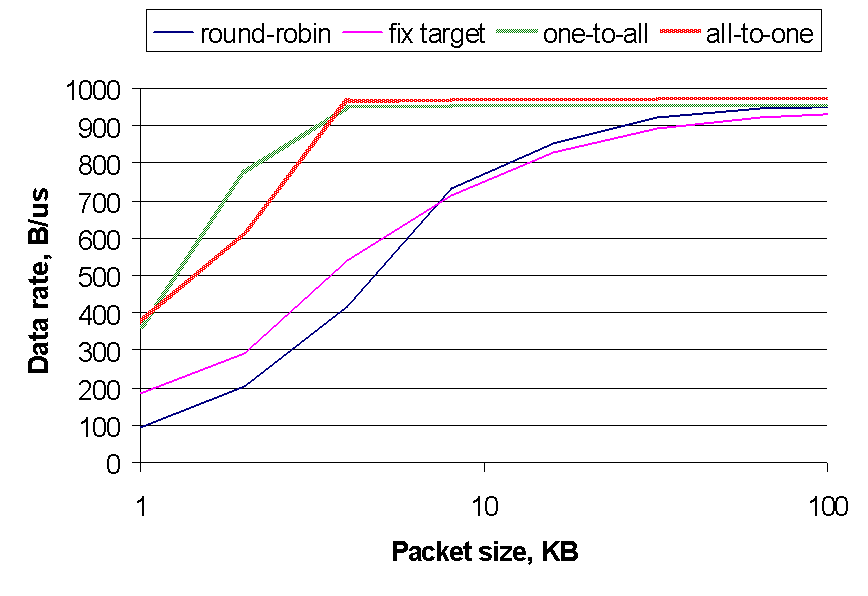
\includegraphics[angle=0,width=.8\textwidth]
{SchMsgRate.png}
\caption{Data transfer rates for message-based scheduled transfer}
\label{fig:ScheduleMessageTransfer}
\end{figure}

The results obtained with RDMA transfer are shown in table \ref{tab:ScheduleRDMATransfer} and 
figure \ref{fig:ScheduleRDMATransfer}.

\begin{table}[htb]
\begin{center}

\caption{Data rates Mb/s for RDMA-based transfers}

\begin{tabular}{|r|c|c|c|c|}\hline

 Buffer  &  Round-robin & Fixed target & One-to-all & All-to-one \\ \hline
    1K  & 110 & 303 & 194 & 320 \\ \hline
    2K  & 214 & 563 & 389 & 596 \\ \hline
    4K  & 424 & 766 & 950 & 966 \\ \hline
    8K  & 788 & 832 & 953 & 969 \\ \hline
   16K  & 888 & 888 & 954 & 970 \\ \hline
   32K  & 941 & 928 & 955 & 971 \\ \hline
   64K  & 951 & 945 & 956 & 972 \\ \hline
  128K  & 954 & 945 & 956 & 972 \\ \hline

\end{tabular}
\end{center}
\label{tab:ScheduleRDMATransfer}
\end{table}

\begin{figure}[htb]
\centering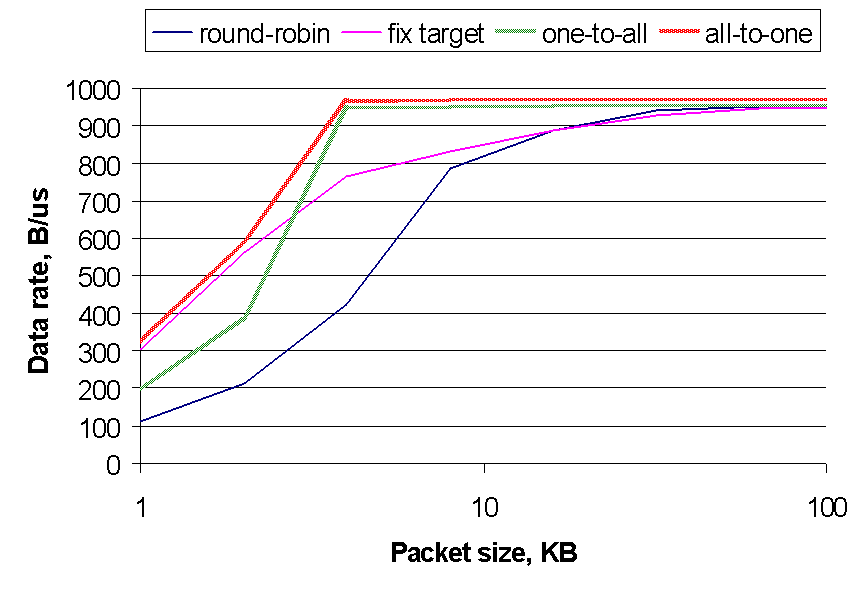
\includegraphics[angle=0,width=.8\textwidth]
{SchRdmaRate.png}
\caption{Data transfer rates for RDMA-based scheduled transfer}
\label{fig:ScheduleRDMATransfer}
\end{figure}

As can be seen the only difference between message-based and RDMA transfer 
shows up in the range of small packet sizes, 
where RDMA transfer is two times faster. 

\subsection{``Chaotic'' data transfer}

This is opposite to the scheduled data transfer approach. 
In this mode no synchronisation between nodes is applyed - 
each node tries to send as many packet as possible in all directions. 
In practice it means, that the output queue for 
each point-to-point connection is kept always filled. 
Still, one should take care, that the receiving queue size is not less
than the sending one. 

It turns out that the transfer rates depend from queue size allocated for receiving and sending data. 
The sending queue size was fixed to 10 entries. 
For the receiving queue three different values were tested: \\
11 entries (marked as ``queue11''), \\
20 entries (marked as ``queue20'') and\\ 
100 entries (marked as ``queue100''). \\
The results of tests are shown in table \ref{tab:ChaoticTransfer} and 
figure \ref{fig:ChaoticTransfer}.

\begin{table}[htb]
\begin{center}

\caption{Data rates for chaotic transfers (to be changed)}

\begin{tabular}{|r|c|c|c|c|}\hline

 Buffer  &  ``queue11'' & ``queue20'' & ``queue100'' \\ \hline
    1K  &  93 & 142 & 266 \\ \hline
    2K  & 131 & 168 & 551 \\ \hline
    4K  & 180 & 490 & 755 \\ \hline
    8K  & 279 & 909 & 839 \\ \hline
   16K  & 930 & 948 & 907 \\ \hline
   32K  & 955 & 957 & 938 \\ \hline
   64K  & 960 & 959 & 967 \\ \hline
  128K  & 962 & 962 & 959 \\ \hline

\end{tabular}
\end{center}
\label{tab:ChaoticTransfer}
\end{table}

\begin{figure}[htb]
\centering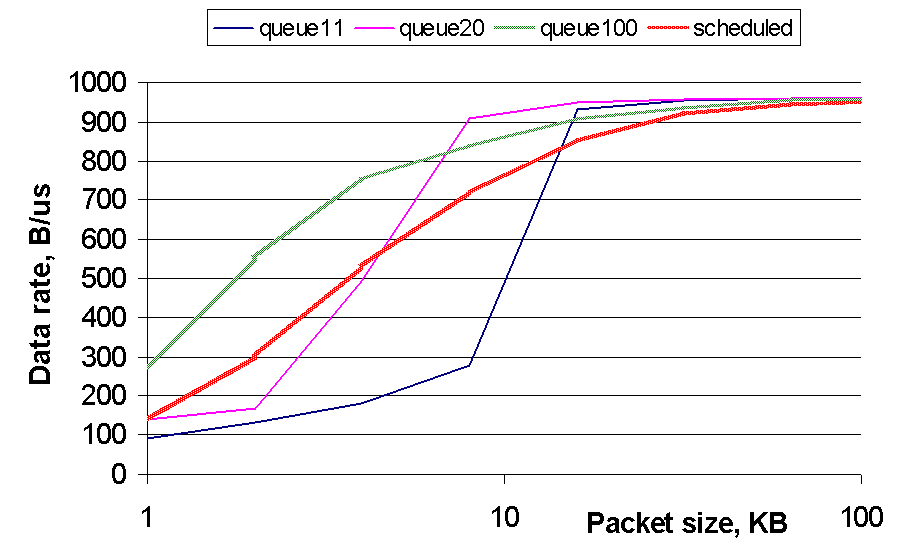
\includegraphics[angle=0,width=.8\textwidth]
{ChaoticRate.png}
\caption{Data transfer rates for chaotic transfer compared with scheduled approach}
\label{fig:ChaoticTransfer}
\end{figure}

One can see, that for small packet sizes large receiving queues provide better performance.
But for buffer sizes above 8 KBytes medium and even small queue sizes gave better performance. 

On the figure \ref{fig:ChaoticTransfer} one can also see a comparison of ``chaotic'' 
transfers with scheduled ones.
From first glance one expects that the data rate achievable by ``chaotic'' transfers must be
less compare to scheduled traffic. But tests with our small 4-nodes traffic show, 
that the ``chaotic'' approach provides much better 
performance for small packet size. 

To better understand such behaviour the transfer rates as function of time were investigated.
One can see on figure \ref{fig:ChaoticTimeDepen} that data rates, 
measured for 1Kb buffer transfers for each connection,
change with time. The variation for a single connection can be estimated as about 50\%.
There are also periods, when total throughput drops down. At the same time measurements, done for
16Kb buffers show practically no any significant variation neither for single connections 
nor for the sum tranfer rate.

Several explanations could be found for this effect. 
Physiscally, one has a single InfiniBand cable, 
connecting host PC and switch, where three virtual connections are established.
On a host PC each connection is treated similary.
But it seems that on the switch side this is not the case. The switch buffers as many data 
as it can and push them further with its own algorithms. 
As a result one sees variations of the transfer rate over single connections and even
of overall performance.
It seems that scheduled data transfers can only work on the lower limit, 
which leads to significant loss of practically achievable
performance for small packet size.

\begin{figure}[htb]
\centering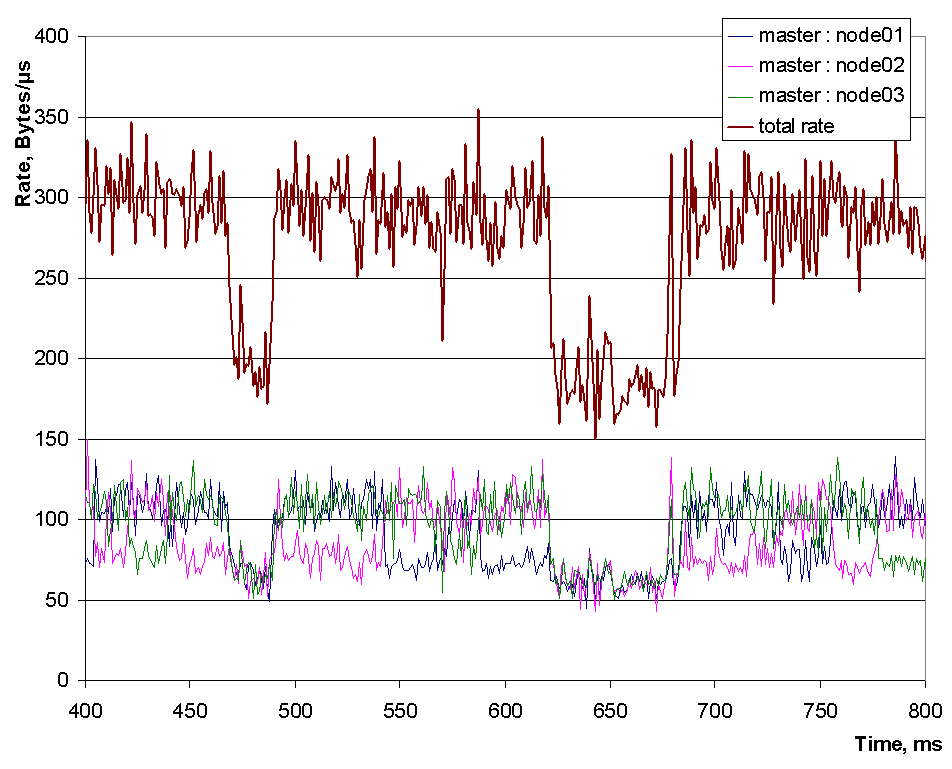
\includegraphics[angle=0,width=.8\textwidth]
{ChaoticTimeDepen.png}
\caption{Dependency of data transfer rates over P2P connection over time. Buffer 1Kb}
\label{fig:ChaoticTimeDepen}
\end{figure}


The advantage of using ``chaotic'' transfers
is that one does not need an exact timing for send operations and
can use uDAPL wait functions instead polling over incoming events. 
This reduces the CPU usage, especially for 
big packet sizes, when the number of I/O operations is moderate. 

``Chaotic'' schedule also was tested with non-fixed packet size. 
Packet sizes were varing around an average value by $\pm50\%$.
No significant difference with results for fixed-packet sizes were observed.


\subsection{Concequence of firmware update}

After firmware update on host adapter and InfiniBand switch test results were improved.
First of all, scheduled transfer with small packets size gets practically the same perfromance as 
in chaotic transfer. Second, irregularity in the data rates during chaotic transfer practially
dissapear. 

\begin{figure}[htb]
\centering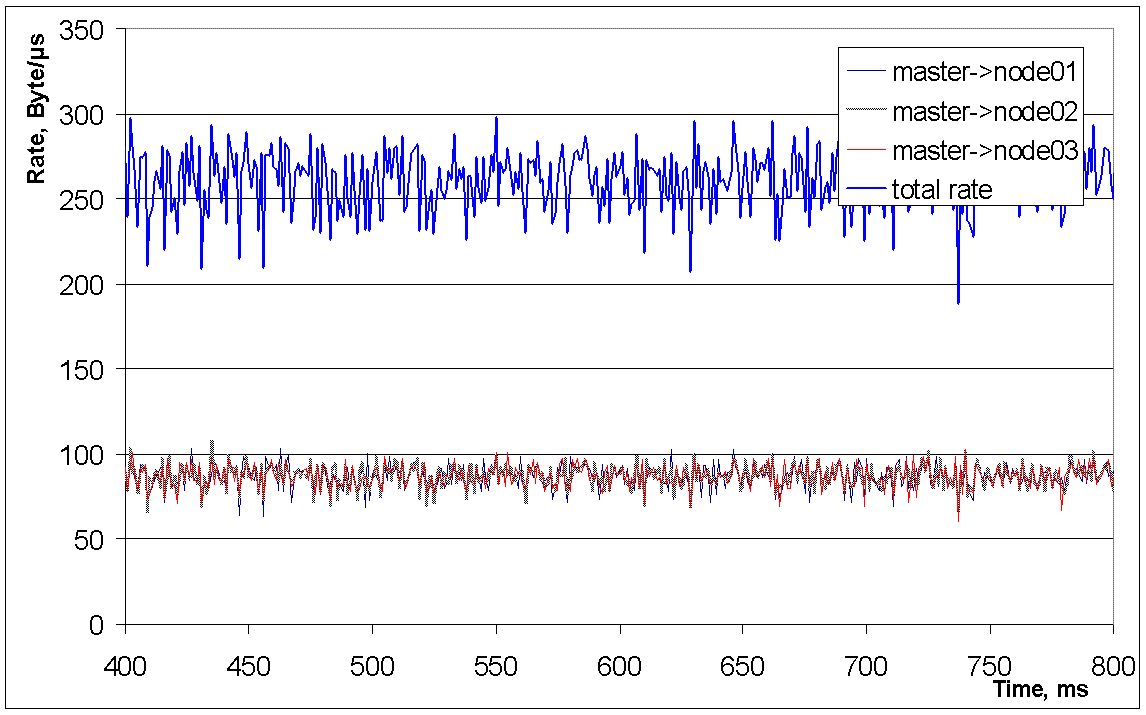
\includegraphics[angle=0,width=.8\textwidth]
{ChaoticTimeDepenNew.png}
\caption{Dependency of data transfer rates over P2P connection over time after firmware upgrade. Buffer 1Kb}
\label{fig:ChaoticTimeDepenNew}
\end{figure}

On figure \ref{fig:ChaoticTimeDepenNew} one can see, that transfer rate variation remains arround 
same average value and does not droped any longer. 

